\chapter{Introduction}

\section{Overview}

For decades, agriculture has been associated with the production of essential 
food crops. Nowadays, agriculture above and beyond farming includes forestry, 
dairy, fruit cultivation, poultry, beekeeping, mushroom, arbitrary, etc. Today, 
processing, marketing, and distribution of crops and livestock products, etc. 
Are all acknowledged as part of current agriculture? Thus, agriculture could 
be referred to as the production, processing, promotion, and distribution of 
agricultural products. Agriculture plays a critical role in the entire life 
of a given economy.

Agriculture is the backbone of the economic system of every country. 
In addition to providing food and raw material, agriculture provides 
employment opportunities to a very high percentage of the population. \\

In most parts of the world, agriculture is an essential source of livelihood,
which entails hard work, but it contributes to the nation's food safety and 
health. Agriculture was the primary source of the economy before the industrial 
revolution. With the many coming up trade options, many people depend on agriculture 
as the main source of income. Agriculture is the most peaceful and environmentally 
friendly method. It is a very reliable source of life for humanity, as well as 
one of the honest sources of income. Many people from developing countries rely 
for their livelihood on agriculture. \\

One of the prime factors in ensuring consistent marketing of crops is product quality. 
For many crops, the main indicator of product quality from the customer's perspective 
is crop ripeness and health. Also, one of the most worrying issues for producers is 
the product's appearance as it has a high influence on the product's quality and consumer 
preferences. Fruit ripening is characterized by the development of color, flavor, texture, 
and aroma. The actual time from anthesis until full maturity can vary tremendously among 
species/cultivars due to genetic and environmental differences. Even between fruit on the 
same plant, fruit development, and ripening can take more or less time depending on local 
microclimate conditions and differences in sink/source relations within the plant. \\

In addition, when a fruit is harvested, the time of anthesis of a particular fruit is 
generally unknown, as is its full history. Monitoring and controlling fruit and vegetable 
ripeness has become a very important issue in the crops industry since ripeness is perceived 
by customers as the main quality indicator. Also, the product's appearance is one of the most 
worrying issues for producers as it has a highl influence on the product's quality 
and consumer preferences. However, up to this day, optimal harvest dates and 
prediction of storage life are still mainly based on subjective interpretation 
and practical experience. \\

Plant pests and diseases affect crops, causing significant losses to farmers 
and threatening food security. The spread of plant pests and diseases has 
increased dramatically in recent years. Globalization, trade, and climate 
change, as well as reduced resilience in production systems due to decades 
of agricultural intensification, have all played a part. Plant pests and 
diseases can quickly spread to several countries and reach epidemic proportions. 
Outbreaks and upsurges can cause huge losses to crops and pastures, threatening 
the livelihoods of vulnerable farmers and the food and nutrition security of 
millions at a time \cite{dir19}. \\[5pt]

\begin{figure}[H]
        \centering
        \begin{tabular}{cccc}
            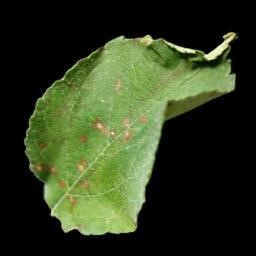
\includegraphics[width=3.2cm]{photos/chapter01/1.jpg}   & 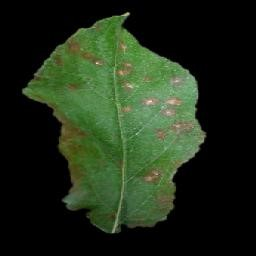
\includegraphics[width=3.2cm]{photos/chapter01/2.jpg}
            & 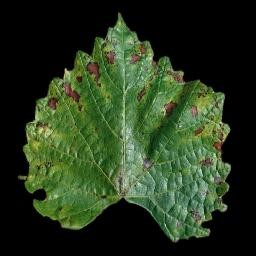
\includegraphics[width=3.2cm]{photos/chapter01/3.jpg} & 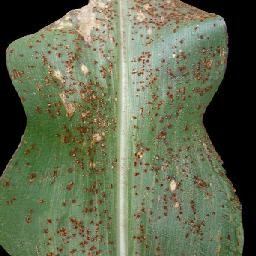
\includegraphics[width=3.2cm]{photos/chapter01/4.jpg} \\
            (a) Apple & (b) Apple & (c) Grape & (d) Corn \\[6pt]
        \end{tabular}
        \caption{Plant pests and diseases}
\end{figure}

\noindent
\key{Plant pests and diseases spread in three principal ways:}
\begin{itemize}
    \item trade or other human - migrated movement.
    \item environmental forces - weather and wind borne.
    \item insect or other vector-borne - pathogens.
\end{itemize}

Hence, automation of this process is a big gain at agriculture and industry fields. 
For agriculture, it may be used to develop automatic harvest systems and saving crops 
from damages caused by environmental changes. On the other hand, for industry, it is 
used to develop automatic sorting system or checking the quality of fruits to increase 
customer satisfaction level \cite{bre00}. So, an objective and accurate ripeness and health 
assessment of agricultural crops is important in ensuring optimum yield of high quality 
products. Moreover, identifying physiological and harvest maturity of agricultural crops 
correctly, will ensure timely harvest to avoid cutting of either under- and over-ripe 
agricultural crops \cite{may11, mah21}. \\

Agricultural sustainability can be attained through vision enabled autonomous machines 
that work together as a phenomenon to ensure global food security. The demand for 
efficient as well as reliable food production techniques is rapidly increasing day by 
day. Computer vision tagged with machine learning approaches grabbed considerable 
attention for research to meet this demand through analyzing and understanding the 
input images from humans, robots, drones, sensors, satellites, etc. \\
Began to use computer vision and machine learning as well as deep learning techniques 
for attaining increased agricultural productions. Additionally, with the help of the 
above-mentioned techniques different agricultural activities, such as crop health 
monitoring, weed, disease, pest detection, etc. have also been reviewed to overcome 
the current challenges and explore the future opportunities for smart farming with 
low cost and high efficiency \cite{dir19}.


\section{Problem Definition}

Agricultural crops at greenhouse, fields and storage containers are affected by 
changes at climate such as temperature and humidity levels, etc. These changes can 
cause diseases, loss of nutritional value, over-ripen and changes at texture, 
appearance and flavor and this affect the quality of the agricultural crops. 
Crop diseases are a major threat to food security, but their rapid identification 
remains difficult in many parts of the world due to the lack of the necessary 
infrastructure. Monitor the ripeness process and health of crops is very important 
issue at agricultural and industry. The combination of increasing global smartphone 
penetration and recent advances in computer vision made possible by deep learning 
has paved the way for smartphone-assisted disease diagnosis.


\section{Project Objectives}

The main objectives of this project to be accomplished within 
a timeline and with available resources are:

\begin{enumerate}
    \item Developing an automated helpful system for agriculture that can be useful 
        for farmers, farming lovers, and agricultural companies. It can perform the main agricultural 
        tasks accurately using deep learning to solve the 
        problems faced by farmers such as:
        \begin{enumerate}
            \item Crop identification.
            \item Identification of diseases.
            \item Detection of insects.
            \item Fruit detection.
            \item Ripeness Assessment.
        \end{enumerate}
    \item Early detection of the disease helps farmers to make the right 
        decision about treatment and preventive things such as
        \begin{enumerate}
            \item Fertilizers.
            \item Herbicides.
            \item Insecticides.
        \end{enumerate}
\end{enumerate}

\section{Project Plan}

\begin{itemize}
    \item Building a theoretical concepts background including 
        (Literature review, Survey on similar systems and project proposal).
    \item Choosing specific crops and preparing images dataset.
    \item Studying chosen crops nature and what are the most important 
        features for ripeness assessment and disease recognition?
    \item Studying different deep learning models for classification.
        \begin{enumerate}
            \item Pre-processing and features extraction.
            \item Classifications and decision making
            \item Experimental results and evaluation
        \end{enumerate}
\end{itemize}

\section{Organization}

We structure the rest of this project as follows: 
Chapter (2) presents a survey of some work in this area and related problems in details,
Chapter (3) is an overview of the methods used in the proposed system,
Chapter (4) gives a detailed description of the phases of the proposed classification system,
Experimental results and comparative analysis are discussed in chapter (5), 
Challenges and future trends are presented in chapter (6).

